\RequirePackage[l2tabu, orthodox]{nag}%TODO: Remove this line after checking
%\documentclass[11pt, a4paper,twoside]{scrartcl} % Seminar
\documentclass[technote,a4paper,leqno]{IEEEtran}
\pdfoutput=1

% packages
\usepackage[utf8]{inputenc}
\usepackage[T1]{fontenc}
\usepackage{ae}
\usepackage{tabularx}
\usepackage{amsmath,amssymb}
\usepackage[pdftex]{graphicx}
\usepackage{subfigure}
\usepackage{url}
\usepackage{ifthen}
\usepackage{url}
\usepackage{breakurl}
\usepackage[breaklinks]{hyperref}
\def\UrlBreaks{\do\/\do-}
\usepackage[absolute,overlay]{textpos}
\usepackage{tikz}
\usepackage{csquotes}
\usepackage[english,ngerman]{babel}
\usepackage[headsepline,footsepline,plainheadsepline]{scrpage2}
\usepackage{changepage}
\usepackage[inner=3cm,outer=2.5cm,top=2.5cm,bottom=2cm,includeheadfoot]{geometry}
\usepackage[xindy,toc]{glossaries}
\loadglsentries[main]{glossary}
\makeglossaries

% Packages like in our pixel-wise-street-segmentation
% nameinlink, noabbrev: not supported by arxiv :-(
\usepackage[nameinlink, noabbrev,capitalise]{cleveref} % has to be after hyperref, nthe l.137 ...eam attr{/N 4}  file{sRGBIEC1966-2.1.icmorem, amsthm
\usepackage[binary-units,group-separator={,}]{siunitx}
\sisetup{per-mode=fraction,binary-units=true}
\DeclareSIUnit\pixel{px}
\usepackage{microtype}

\DeclareGraphicsExtensions{.jpg}

% ORCID: http://orcid.org/0000-0002-9178-2970 Teichmann, Marvin
% ORCID: http://orcid.org/0000-0002-6517-1690 Thoma, Martin

\title{The State of the Art in automatic, fixed class, single-image Segmentation}
\author{%
\makebox[.4\linewidth]{Marvin Teichmann\thanks{\IEEEauthorrefmark{1} These authors contributed equally to this work}\IEEEauthorrefmark{1}} % ORCID: http://orcid.org/0000-0002-9178-2970
\and \makebox[.4\linewidth]{Martin Thoma\IEEEauthorrefmark{1}}} % ORCID: http://orcid.org/0000-0002-6517-1690

% arxiv doesn't like \sep
\hypersetup{
    pdfauthor   = {Marvin Teichmann, Martin Thoma},
    pdfkeywords = {semantic segmentation, pixelwise classification, pixel-level classification},
    pdfsubject  = {Segmentation},
    pdftitle    = {The State of the Art in automatic, fixed class, single-image Segmentation},
}

\begin{document}
\selectlanguage{english}
\maketitle
%!TEX root = vorlage.tex

\begin{abstract}
This survey gives an overview over different techniques used for pixel-level
semantic segmentation. It is based on an extensive literature review. Metrics
and datasets for the evaluation of segmentation algorithms, traditional
approaches for segmentation as well as recently published approaches with
convolutional neural networks and typical problematic situations for segmentation
algorithms are examined.
\end{abstract}


%!TEX root = vorlage.tex
% Marvin Teichmann and Martin Thoma
\section{Introduction}\label{sec:introduction}
Semantic segmentation is the task of clustering parts of images together which
belong to the same object. This type of algorithm has several use-cases such as
detecting objects in robotics (TODO: cite), detecting street signs in
self-driving car software (TODO: cite), detecting tumors in medicine (TODO: cite),
detecting medical instruments in operations and distingushing them from
tissue (TODO: cite).

% Pixelwise segmentation is an imporant sub-task of many applications and can
% be applied to support even more applications: Understanding images (TODO:
% Cite paper google automatically labeling images), object detection (TODO:
% Cite a paper probably by Asfour), street detection (TODO: Cite), face
% detection (TODO: cite) and medical instrument detection (TODO: cite) are only
% a couple of the possible applications.

% In many applications speed and accuracy is crucial. In this paper, we
% summarize the current state of semantic segmentation.


Taking a step back, the task of semantic segmentation can be grouped in several
categories:

\begin{itemize}
    \item \textbf{By possible classes}: Are the classes which should be distinguised
          known at the time when the algorithm is developed / trained or might
          there occur several objects which were never seen before?
          \begin{itemize}
              \item Fixed-class: All classes are known at training time.
              \begin{itemize}
                  \item Binary: street/no street.
              \end{itemize}
              \item Open-class: There might be completely new classes
          \end{itemize}
    \item \textbf{By class affiliation of pixels}:
        \begin{itemize}
            \item Single class affiliation: Every pixel belongs to exactly one class. There might
                  be probabilities, but a pixel cannot belong with a 100\%
                  probability to two classes.
            \item Multiple class affiliation: A single pixel might belong to
                  multiple classes. An example is a glass on a table: One
                  knows that the glass is there and it is possible to see the
                  table below / behind. Another example is hair. Mattening
                  methods produce maps which reflect this property for hair.\cite{levin2008spectral}
        \end{itemize}
    \item \textbf{By input data}:
          \begin{itemize}
              \item greyscale / colored
              \item single image (NOTE: we write about this) / time series (NOTE: only mention it)
          \end{itemize}
    \item \textbf{Operation state}:
        \begin{itemize}
            \item completely automatically <-- we write about this type
            \item interactive (e.g. user clicks on background or user makes a
                  coarse segmentation and automatically refinement) as
                  described in
                  \cite{protiere2007interactive,rother2004grabcut}.
            \item active as in
                  \cite{schiebener2011segmentation,schiebener2012discovery} or
                  passive, where the received image cannot be influenced
        \end{itemize}
\end{itemize}

%!TEX root = vorlage.tex

\section{Taxonomy of Segmentation Algorithms}\label{sec:taxonomy}
The computer vision community has published a wide range of segmentation
algorithms so far. Those algorithms can be grouped by the kind of data they
operate on and the kind of segmentation they are able to produce.

The following subsections will give four different criteria by which
segmentation algorithms can be classified.

This survey describes fixed-class (see \cref{subsec:allowed-classes}),
single-class affiliation (see \cref{subsec:class-affiliation}) algorithms which
work on grayscale or colored single pixel images (see \cref{subsec:input-data})
in a completely automated, passive fashion (see \cref{subsec:operation-state}).


\subsection{Allowed classes}\label{subsec:allowed-classes}
Semantic segmentation is a classification task. As such, the classes on which
the algorithm is trained is a central design decision.

Most algorithms work with a fixed set of classes; some even only work on binary
classes like \textit{foreground vs
background}~\cite{4228537,carreira2010constrained} or \textit{street vs no
street}~\cite{bittel2015pixel}.

However, there are also unsupervised segmentation algorithms which do not
distinguish classes at all (see
\cref{subsec:unsupervised-traditional-segmentation}) as well as segmentation
algorithms which are able to recognize when they don't know a class. For
example, in~\cite{gould2008multi} a
\textbf{void class} was added for classes which were not in the training set.
Such a void class was also used in the MSRCv2 dataset (see
\cref{subsubsec:MSRCv2}) to make it possible to make more coarse segmentations
and thus having to spend less time annotating the image.


\subsection{Class affiliation of pixels}\label{subsec:class-affiliation}
Humans do an incredible job when looking at the world. For example, when we see
a glass of water standing on a table we can automatically say that there is the
glass and behind it the table, even if we only had a single image and were not
allowed to move. This means we simultaneously two labels to the coordinates of
the glass: Glass and table. Although there is much more work being done on
\textbf{single class affiliation} segmentation algorithms, there is a
publication about \textbf{multiple class affiliation}
segmentation~\cite{levin2008spectral}. Similarly, recent publications in
pixel-level object segmentation used layered models~\cite{yang2012layered}.

\goodbreak
\subsection{Input Data}\label{subsec:input-data}
The available data which can be used for the inference of a segmentation varies
by application.

\begin{itemize}
    \item \textbf{Grayscale vs colored}: Grayscale images are commonly used in
          medical imaging such as \gls{MR} imaging or ultrasonography whereas
          colored photographs are obviously widespread.
    \item \textbf{Excluding or including depth data}: RGB-D, sometimes also
          called range~\cite{hoover1996experimental} is available in robotics,
          autonomous cars and recently also in consumer electronics such as
          Microsoft Kinect~\cite{6190806}.
    \item \textbf{Single image vs stereo images vs co-segmentation}: Single
          image segmentation is the most wide-spread kind of segmentation, but
          using stereo images was already tried in~\cite{boykov2001fast}. It
          can be seen as a more natural way of segmentation as most mammals
          have two eyes. It can also be seen as being related to having
          depth data.\\
          Co-segmentation as in~\cite{1640859,collins2012random} is the problem
          of finding a consistent segmentation for multiple images. This problem
          can be seen in two ways: One the one hand, it can be seen as the problem
          of finding common objects in at least two images. On the other hand,
          every image after the first can be used as an additional source of
          information to find a meaningful segmentation. This idea can be
          extended to time series such as videos.
    \item \textbf{2D vs 3D}: Segmenting images is a 2D~segmentation task where
          the smallest unit is called a \textit{pixel}. In 3D data, such as
          volumetric X-ray CT images as they were used in~\cite{929615}, the
          smallest unit is called a voxel.
\end{itemize}


\subsection{Operation state}\label{subsec:operation-state}
The operation state of the classifying machine can either be \textbf{active} as
in~\cite{schiebener2011segmentation,schiebener2012discovery} where robots can
move objects to find a segmentation or \textbf{passive}, where the received
image cannot be influenced. Among the passive algorithms, some segment in a
completely \textbf{automatic} fashion, others work in an \textbf{interactive}
mode. One example would be a system where the user clicks on the background or
marks a coarse segmentation and the algorithm finds a fine-grained
segmentation.
\cite{boykov2000interactive,rother2004grabcut,protiere2007interactive}~describe
systems which work in an interactive mode.

%!TEX root = vorlage.tex
% Marvin Teichmann and Martin Thoma
\section{Evaluation and Datasets}\label{sec:evaluation-and-datasets}

%!TEX root = vorlage.tex
% Martin Thoma
\subsection{Quality measures for evaluation}%
\label{subsec:quality-measures}%
A performance measure is a crucial part of any machine learning system, but
there are other measures of quality which matter when segmentation algorithms
are compared. This section gives an overview of those quality measures.


\subsubsection{Accuracy}
Showing the correctness of the segmentation hypotheses is done in most
publications about semantic segmentation. However, there are a couple of
different ways how this accuracy can be displayed. One way to give readers a
first impression of the obtained segmentations is by showing examples such
as~\cref{fig:segmentation-example}.

\begin{figure}
\centering
\subfigure[Example Scene]{
  \label{fig:segmentation-example-scene}
  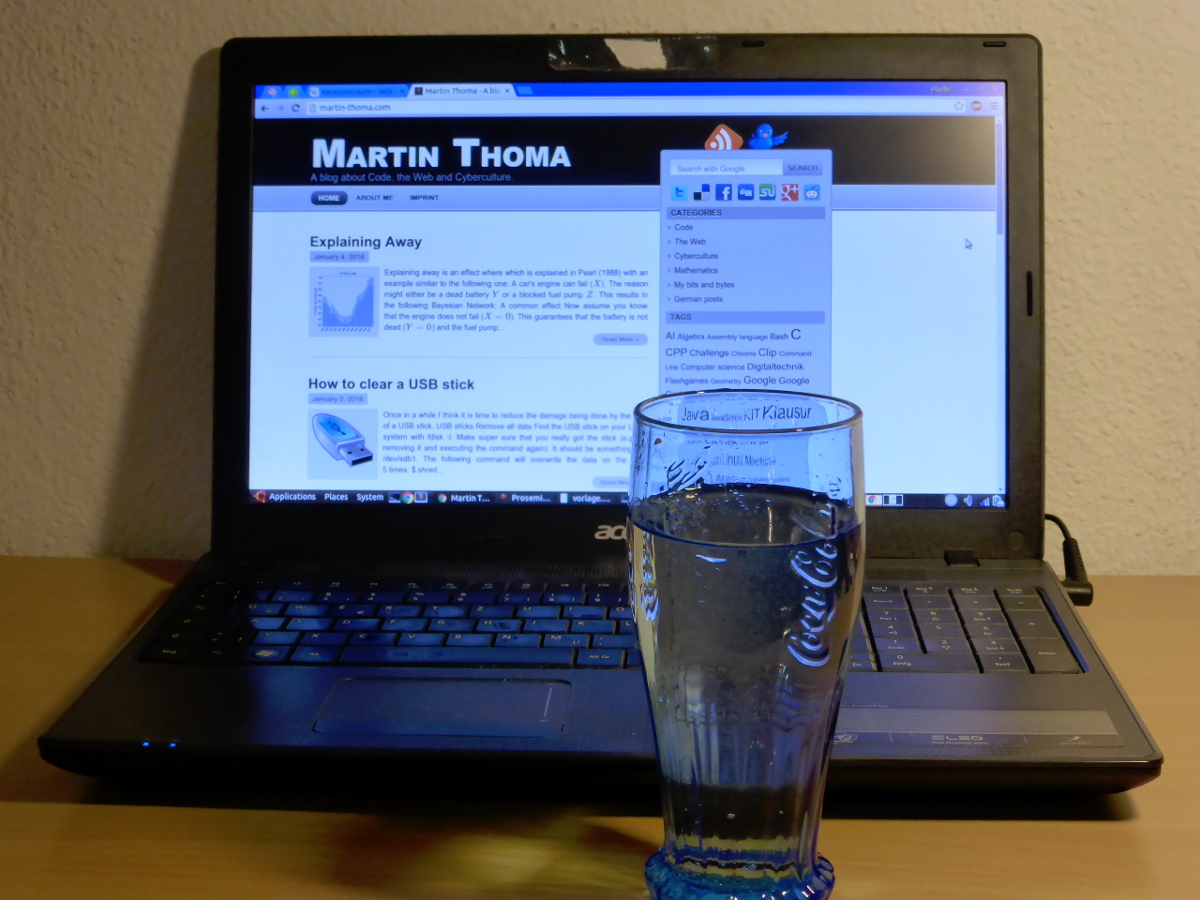
\includegraphics[width=0.45\linewidth, keepaspectratio]{figures/image-segmentation-example.jpg}
}%
\subfigure[Visualization of a found segmentation]{
  \label{fig:segmentation-example-seg}
  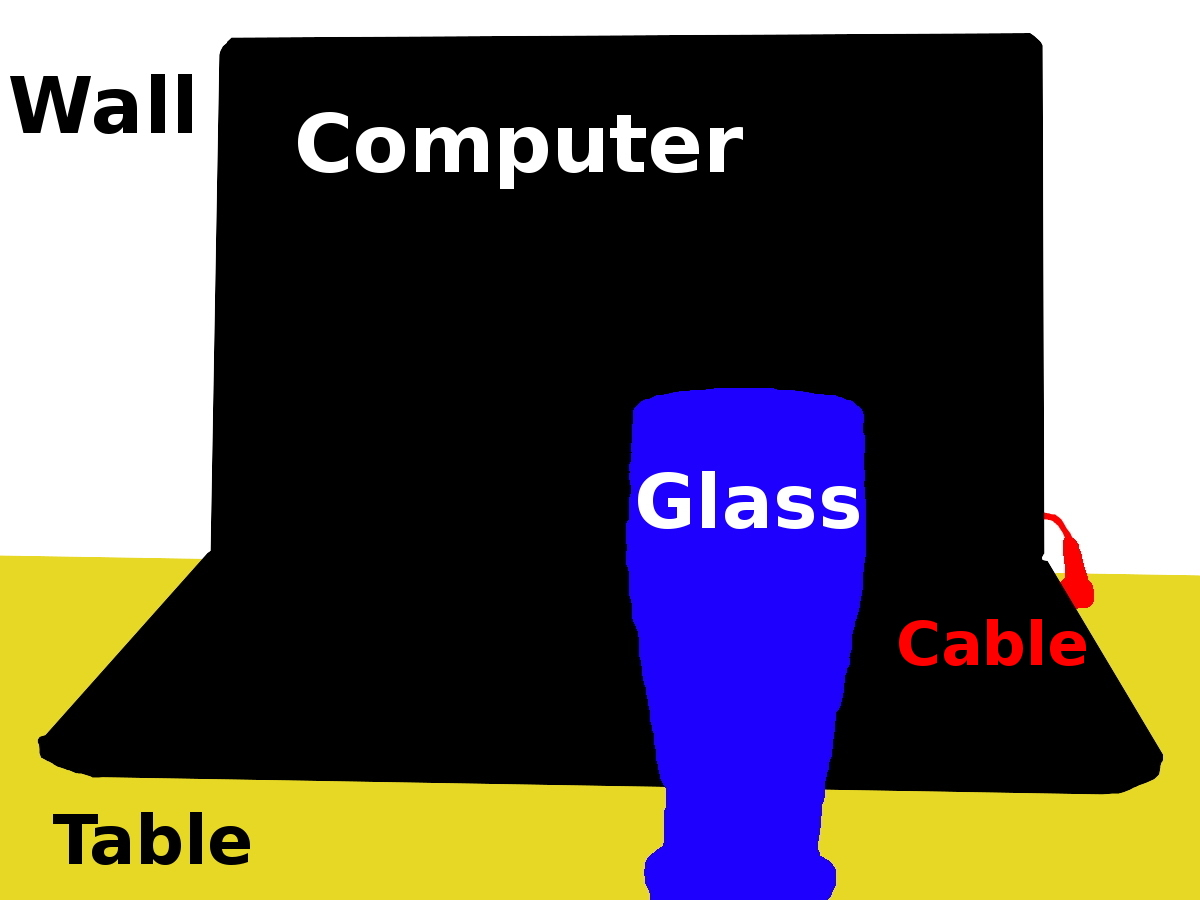
\includegraphics[width=0.45\linewidth, keepaspectratio]{figures/image-segmentation-example-segmented.jpg}
}
\caption{An example of a scene and a possible visualization of a found segmentation.}
\label{fig:segmentation-example}
\end{figure}

However, this can only support the explanation of particular problems or
showcase special situation. For meaningful information about the overall
accuracy, there are a couple of metrics.

For this section, let $k \in \mathbb{N}$ be the number of classes, $n_{ij} \in
\mathbb{N}_0$ with $i,j \in 1, \dots, k$ be the number of pixels which belong to
class~$i$ and were labeled as class~$j$. Let $t_i = \sum_{j=1}^k n_{ij}$ be the
total number of pixels of class~$i$.

One way to compare segmentation algorithms is by the pixel-wise accuracy of the
predicted segmentation as done in many publications
\cite{shotton2006textonboost,csurka2008simple,long2014fully}. This is also
called per-pixel rate and defined as $\frac{\sum_{i=1}^k n_{ii}}{\sum_{i=1}^k
t_i}$. Taking the pixel-wise classification accuracy has two major drawbacks:

\begin{problemnr}
    \item \label{item:problem-large-regions} Tasks like segmenting images for self-driving cars have large regions
          which have one class. This makes achieving classification accuracies
          of more than \SI{30}{\percent} with a priori knowledge only possible.
    \item \label{item:problem-labeling-granularity} The manually labeled images
          could have a more coarse labeling. For example, a human classifier
          could have labeled a region as
          \enquote{car} and the algorithm could have split that region into
          the general \enquote{car} and the more specific \enquote{wheel of a
          car}
\end{problemnr}
\goodbreak
Three accuracy metrics which do not suffer from
\cref{item:problem-large-regions} are used in~\cite{long2014fully}:\nobreak%
\begin{itemize}
    \item \textit{mean accuracy}: $\frac{1}{k} \cdot \sum_{i=1}^n \frac{n_{ii}}{t_i}$
    \item \textit{mean intersection over union}: \hfill\\$\frac{1}{k} \cdot \sum_{i=1}^k \frac{n_{ii}}{t_i + \sum_{j=1}^k n_{ji}-n_{ii}}$
    \item \textit{frequency weighted intersection over union}:
          ${({\sum_{p=1}^k t_p})}^{-1} \sum_i \frac{t_i n_{ii}}{t_i + \sum_{j=1}^k n_{ji} - n_{ii}}$
\end{itemize}

Another problem might be pixels which cannot be assigned one of the known
classes. For this reason, \cite{shotton2006textonboost} makes use of a void
class. This class gets completely ignored for all quality measures. Hence the
total number of pixels is assumed to be $\text{width} \cdot \text{height} - \text{number of void pixels}$.

One way to deal with \cref{item:problem-large-regions} and
\cref{item:problem-labeling-granularity} is giving a confusion matrix as
done in \cite{shotton2006textonboost}. However, this approach is not feasible
if many classes are given.


A lot of other measures for the accuracy of segmentations were proposed for
non-semantic segmentation. One of those accuracy measures is \textit{Normalized
Probabilistic Rand} (NPR) index which was introduced in
\cite{unnikrishnan2005measure} and evaluated in~\cite{celebi2009improved}
on dermoscopy images. Other non-semantic segmentation measures were introduced
in~\cite{martin2001database}, but the reason for creating them seems
to be to deal with the under-defined task description of non-semantic
segmentation. These accuracy measures try to deal with different levels of
coarsity of the segmentation. This is much less of a problem in semantic
segmentation and thus those measures are not explained here.

The $F$-measure is useful for binary classification task such as the KITTI road
segmentation benchmark~\cite{Fritsch2013ITSC} or crypt segmentation as done
by~\cite{cohen2015memory}. It is calculated as \enquote{the harmonic mean of
the precision and recall}~\cite{pantofaru2005comparison}:
\[F_\beta = (1+\beta)^2 \frac{\text{tp}}{(1+\beta^2)\cdot \text{tp}+ \beta^2 \cdot \text{fn} + \text{fp}}\]
where $\beta=1$ is chosen in most cases and \texttt{tp} means \textit{true
positive}, \texttt{fn} means \textit{false negative} and  \texttt{fp} means
\textit{false positive}.


\subsubsection{Speed}%
\label{subsubsec:speed-quality-measure}%
A maximum upper bound on the execution time for the inference on a single image
is a hard requirement for some applications. For example, in the case of
self-driving cars an algorithm which classifies pixel as street or no-street
and thus makes a semantic segmentation, every image needs to be processed
within \SI{20}{\milli\second}~\cite{bittel2015pixel}.

Most papers do not give exact values for the time their application needs. One
reason might be that this is very hardware, implementation and in some cases
even data specific. For example, \cite{hoover1996experimental} notes that their
algorithm needs \SI{10}{\second} on a Sun SparcStation~20. The fastest CPU ever
produced for this system had~\SI{200}{\mega\hertz}. Comparing this directly
with results which were obtained using an Intel~i7-4820K with
\SI{3.9}{\giga\hertz} would not be meaningful.

However, it does still make sense to mention the execution time as well as the
hardware in individual papers. This gives the interested reader the possibility
to estimate how difficult it might be to adjust the algorithm to work in the
required time-constraints. Also, it should be noted if the algorithm can be
executed in parallel as standard \glspl{GPU} on the consumer market can execute
up to 256~kernels in parallel.

% The \gls{CRF} approach presented in \cite{shotton2006textonboost} takes
% approximately three minutes to segment per image on a \SI{2.1}{\giga\hertz}
% machine with \SI{2}{\giga\byte} memory.


\subsubsection{Stability}%
\label{subsubsec:stability-quality-measure}%
The stability of segmentation is a desirable quality measure. One the one hand,
there are some variants of images like slight blurring, Gaussian noise and
similar which should not change the segmentation at all. Also, two images which
show a slight change in perspective should also only result in slight changes
in the segmentation~\cite{pantofaru2005comparison}.

Another desirable stability criterion is parameter choice. If the
segmentation algorithm has hyperparameters, then slightly changing those should
also only result in minor differences of the resulting
segmentations~\cite{pantofaru2005comparison}.


\subsubsection{Memory usage}
Peak memory usage matters when segmentation algorithms get used in devices like
smartphones or cameras, or when the algorithms have to finish in a given time
frame, run on the \gls{GPU} and consume so much memory for single image
segmentation that only the latest graphic cards can be used. However, no
publication we found mentioned the peak memory usage.

%!TEX root = vorlage.tex
% Marvin Teichmann
\subsection{Datasets}


%!TEX root = vorlage.tex
% Martin Thoma
\section{Traditional Approaches}\label{sec:traditional-approaches}

Image segmentation algorithms which use traditional approaches, hence don't
apply neural networks and make heavy use of domain knowledge, are wide-spread
in the computer vision community. This section discribes the most popular ones
and discusses their respective advantages in
\cref{subsec:traditional-approaches-discussion}.

\subsection{$k$-Means}\label{subsec:k-means}

\begin{itemize}
    \item Represent every pixel of the image as a vector (x, y, r, g, b, h, s,
          v, ...).
    \item Define distance function which weights the components
\end{itemize}


\subsection{Watershed Algorithm}\label{subsec:watershed}

\begin{itemize}
    \item Apply to image intensity gives some long superpixels
    \item apply to image gradient magnitude gives rounder superpixels
\end{itemize}

% http://docs.opencv.org/master/d3/db4/tutorial_py_watershed.html#gsc.tab=0
% http://docs.opencv.org/master/d2/dbd/tutorial_distance_transform.html#gsc.tab=0


\subsection{Mean Shift Algorithm}\label{subsec:mean-shift}
The mean shift algorithm was introduced by~\cite{comaniciu2002mean} for
segmentation tasks. The algorithm first applies mean shift filtering on the
original image data and then clusters the remaining points.

TODO: Understand this algorithm. Use \cite{comaniciu2002mean} and
\cite{pantofaru2005comparison} for it.


\subsection{Graph Based Image Segmentation}\label{subsec:graph-based-image-segmentation}
\href{http://cs.brown.edu/~pff/segment/}{cs.brown.edu}
See \cite{felzenszwalb2004efficient}.

TODO: See also \cite{pantofaru2005comparison} for another description.

EDISON is a publicly available software for mean shift segmentation.\cite{christoudias2002synergism}


\subsection{Random Walks}
NOT supervised hence not semantic?!?

Notes from \cite{meilpa2001learning}:

\begin{itemize}
    \item Normalized Cut (see \cite{shi2000normalized}) seems to be a special
          case of this
    \item Seems to be a \enquote{spectral method}
    \item This is pairwise clustering. Clusters points which are similar and
          optimize e.g. for maximum total intracluster similarity. In contrast,
          to statistical clustering which assumes a probabilistic model which
          generates the data, this only defines a similarity function.
    \item Spectral clustering is a similarity based method. Spectral clustering
          methods use eingenvalues / eigenvectors of the matrix obtained by the
          similarity function.
\end{itemize}


\subsection{Conditional Random Fields}
\Glspl{CRF} were applied in \cite{shotton2006textonboost}.

\subsection{Pre-processing}\label{subsec:preprocessing}
A typical image is opened in RGB color space, but depending on the classifier
and the problem another color space might result in better segmentations. RGB,
YcBcr, HSL, Lab and YIQ are some examples used by \cite{cohen2015memory}.

\Gls{PCA} is applied by~\cite{chen2011pixel} to reduce the dimensionality of
the feature space.

\subsection{Post-processing methods}\label{subsec:post-processing-methods}
Post-processing methods are an important part of traditional pixel-level
segmentation approaches. Active contour models are one example of a
post-processing method~\cite{kass1988snakes}.


\subsection{Discussion}\label{subsec:traditional-approaches-discussion}
According to \cite{pantofaru2005comparison}, the mean shift algorithm produces
segmentations that correspond well to human perception, but it is sensitive to
its parameters. Depending on them, different granularities of the segmentation
can be achieved. \cite{pantofaru2005comparison} draws the conclusion, that
the segmentations found by the graph based image segmentation approach
in \cite{felzenszwalb2004efficient} are inferior to the segmentations found
by the mean shift algorithm described in \cite{comaniciu2002mean}.

%!TEX root = vorlage.tex

\section{Neural Networks for Semantic Segmentation}\label{sec:nn}

Artificial neural networks are classifiers which are inspired by neurons.
Every single neuron has some inputs which it sums up, applies a so called
\textit{activation function} to it and gives an output. Those neurons can take
either a feature vector as input or the output of other neurons. In this way,
they build up feature hierarchies.

The parameters they learn are the weights. They get learned by gradient
descent. To do so, an error function --- usually cross-entropy or mean squared
error --- is necessary. For the gradient descent algorithm, one sees the
labeled training data as given, the weights as variables and the error function
as a surface in this weight-space. Minimizing the error function in the weight
space adapts the neural network to the problem.

There are lots of ideas around neural networks like regularization, better
optimization algorithms, automatically building up architectures, design
choices for activation functions. I will not go into detail here, but I want to
outline some of the mayor breakthroughs.

\Glspl{CNN} are neural networks which learn image filters. They drastically
reduce the number of parameters which have to be learned while being still
general enough for the problem domain of images. This was shown by Alex
Krizhevsky~et~al. in~\cite{krizhevsky2012imagenet}. One major idea was a clever
regularization called \textit{dropout training}, which set the output of neurons
while training randomly to zero. Another contribution was the usage of an activation
function called \textit{rectified linear unit}:
\[\varphi_{\text{ReLU}}(x) = \max(0, x)\]
Those are much faster to train than the commonly used sigmoid activation functions
\[\varphi_{\text{Sigmoid}}(x) = \frac{1}{e^{-x} + 1}\]
Krizhevsky~et~al. implemented those ideas and ran it participated in the
\gls{ILSVRC}. The best other system, which used SIFT features and Fisher
Vectors, had a performance of about \SI{25.7}{\percent} while the network by
Alex Krizhevsky~et~al. got \SI{17.0}{\percent} error rate on the ILSVRC-2010.
As a preprocessing step, they downsampled all images to a fixed
size of $\SI{256}{\pixel} \times \SI{256}{\pixel}$ before they fed the features
into their network. This network is commonly known as \textit{AlexNet}.

Another notable paper is~\cite{long2014fully}. The algorithm presented there
makes use of a classifying network such as AlexNet, but applies the complete
network as an image filter. This way, each pixel gets a probability
distribution for each of the trained classes. By taking the most likely class,
a semantic segmentation can be done with arbitrary image sizes.

A very recent publication by Dai~et~al.~\cite{dai2015instance} showed that
segmentation with much deeper networks is possible and achieves better results.

More detailed explanations to neural networks can be found in (TODO: Marvins
publication).

%!TEX root = vorlage.tex

\section{Possible Problems in the Data for Segmentation algorithms}%
\label{sec:problems}

Different segmentation workflows have different problems. However, there are
a couple of special cases which should be tested. Those cases might not occur
often in the training data, but it could still happen in the productive system.

I am not aware of any systematic work which examined the influence of problems
such as the following.

\subsection{Lens Flare}
Lens flare is the effect of light getting scattered in the lens system of the
camera. The testing data set of the KITTI road evaluation
benchmark~\cite{Fritsch2013ITSC} has a couple of photos with this problem.
\Cref{fig:lens-flare} shows an extreme example of lens flare.


\subsection{Vignetting}
Vignetting is the effect of a photograph getting darker in the corners. This
can have many reasons, for example filters on the camera blocking light at the
corners.


\begin{figure}
\centering
\subfigure[Lens Flare\newline Image by \cite{image:wikipedia:lens-flare} \label{fig:lens-flare}]{
  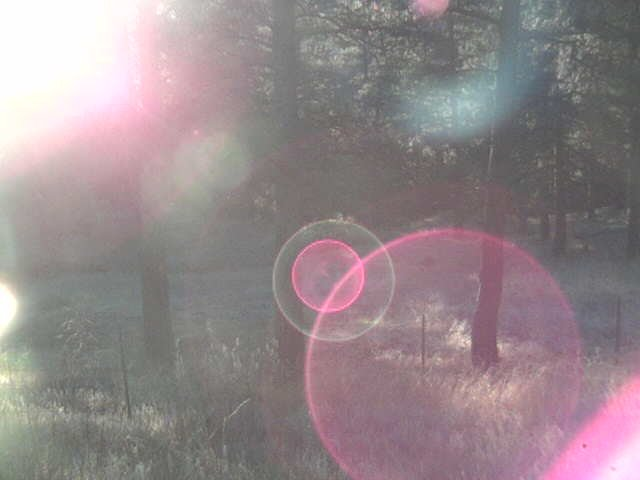
\includegraphics[width=0.45\linewidth, keepaspectratio]{figures/CCTV-Lens-flare.jpg}
}%
\subfigure[Vignetting\newline Image by \cite{image:wikipedia:vignetting} \label{fig:Vignetting}]{
  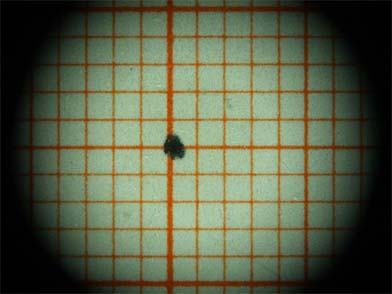
\includegraphics[width=0.45\linewidth, keepaspectratio]{figures/Randabschattung-Mikroskop-Kamera-6.JPG}
}
\subfigure[Smoke by cauterization\newline Image by \cite{giannarou2013probabilistic} \label{fig:smoke}]{
  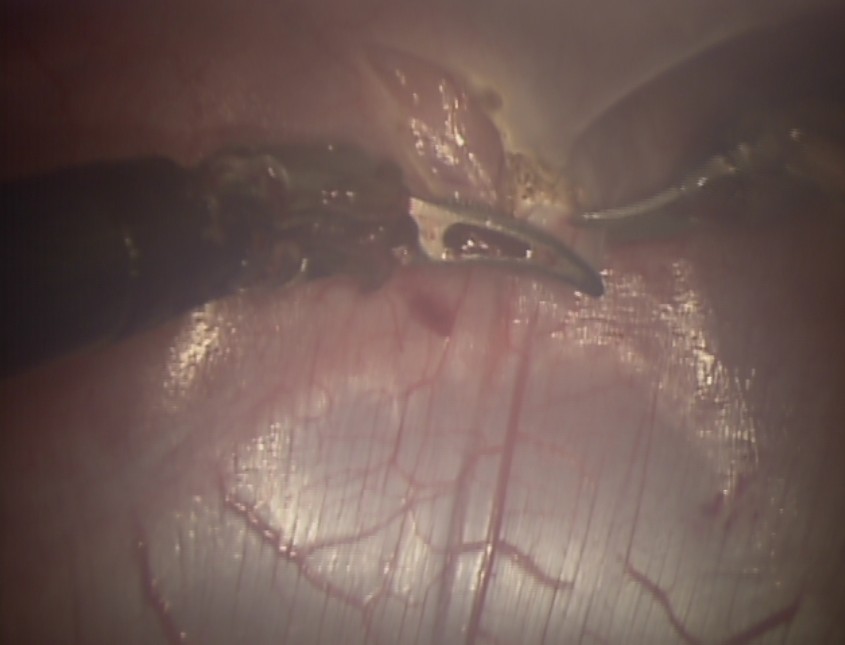
\includegraphics[width=0.45\linewidth, keepaspectratio]{figures/smoke-capture1-033.png}
}%
\subfigure[Camouflage\newline Image by \cite{image:wikipedia:camouflage} \label{fig:camouflage}]{
  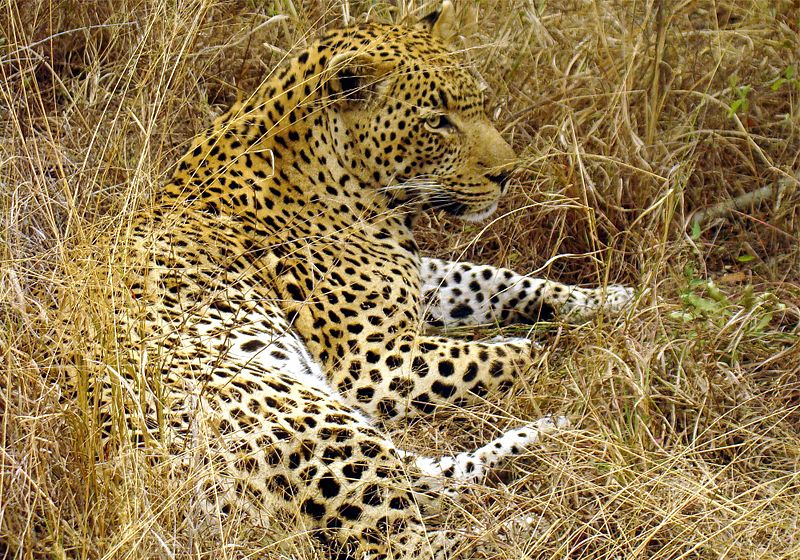
\includegraphics[width=0.45\linewidth, keepaspectratio]{figures/great-male-leopard.JPG}
}
\subfigure[Transparency \label{fig:transparency-glass}]{
  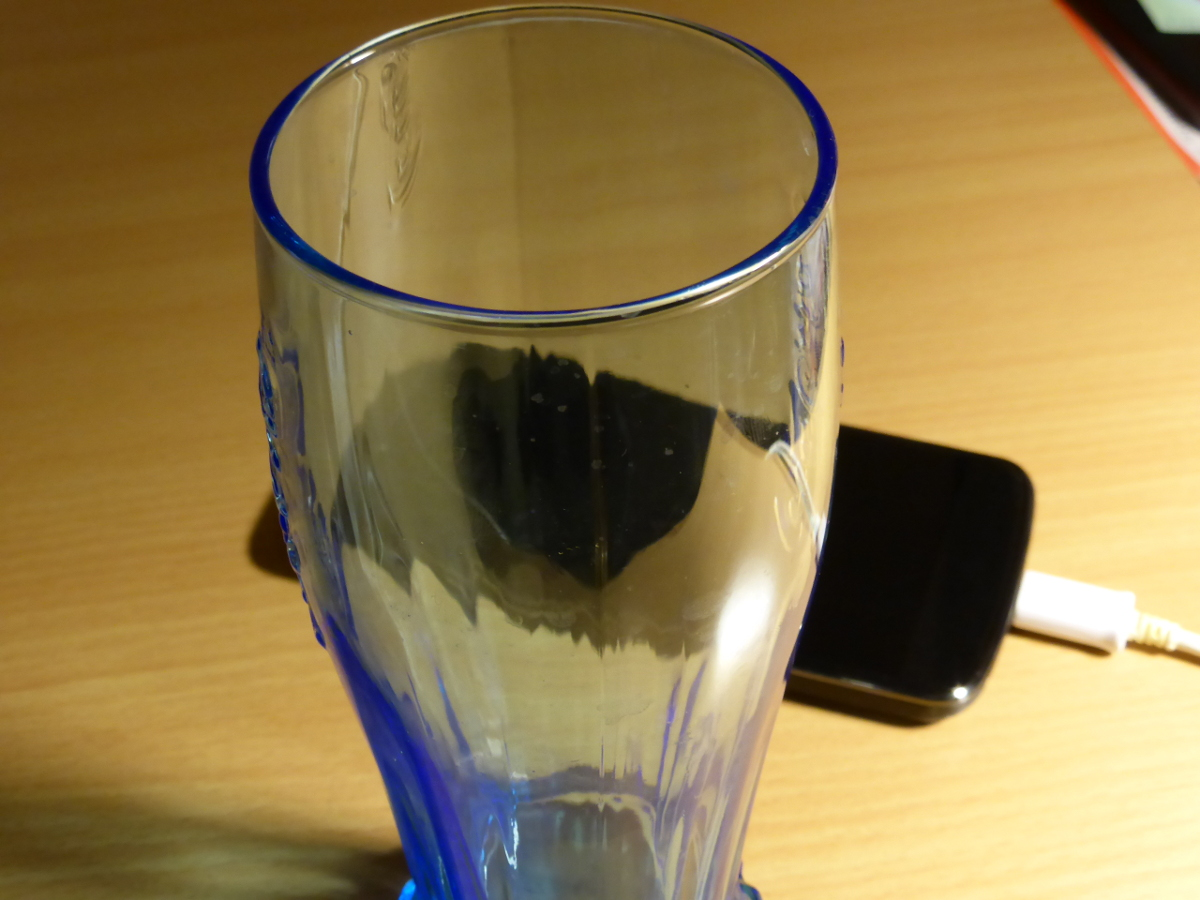
\includegraphics[width=0.45\linewidth, keepaspectratio]{figures/glass-smartphone-table-2.jpg}
}%
\subfigure[Viewpoint \label{fig:viewpoint}]{
  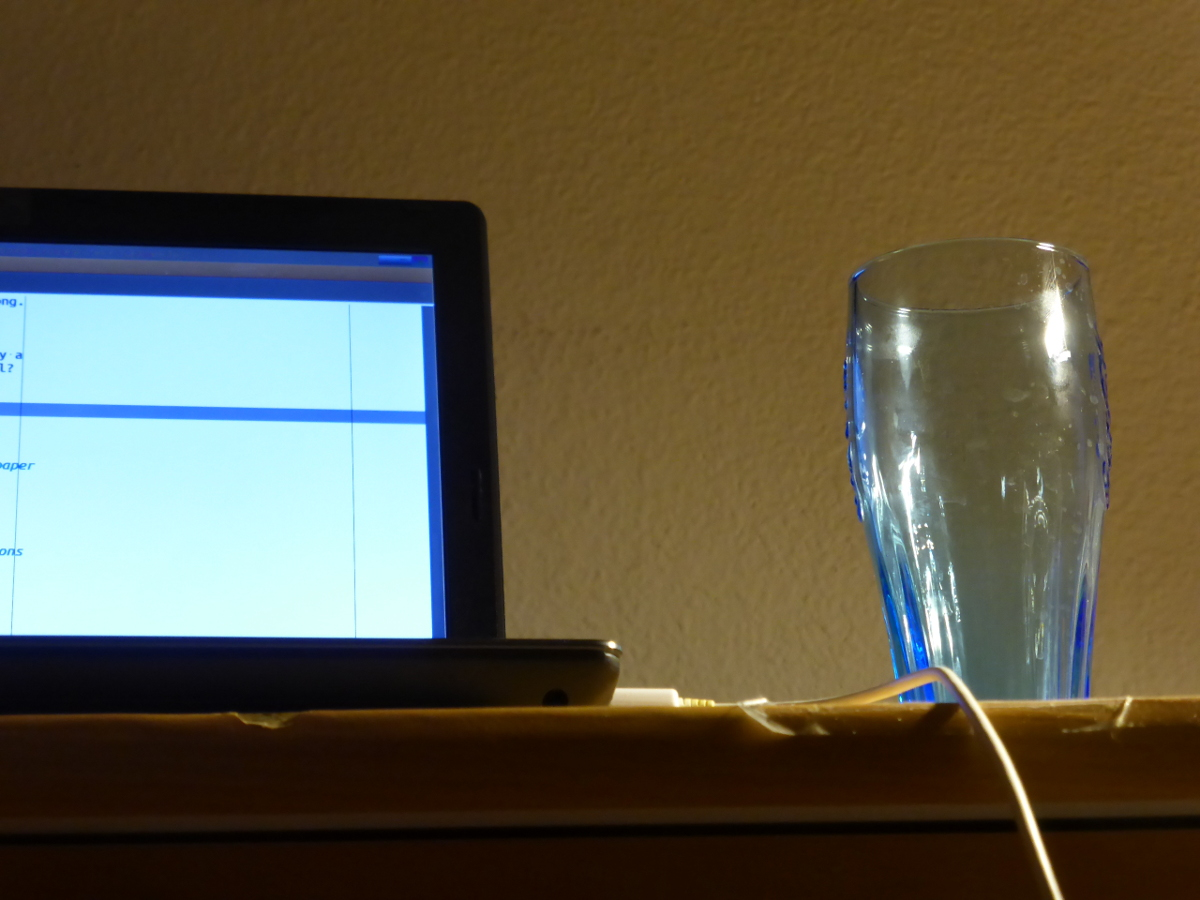
\includegraphics[width=0.45\linewidth, keepaspectratio]{figures/unusual-viewpoint-glass-computer.jpg}
}
\caption{Examples of images which might cause semantic segmentation systems to fail.}
\label{fig:test}
\end{figure}


\subsection{Blurred images}
Images can be blurred for a couple of reasons. A problem with the lenses
mechanics, focusing on the wrong point, too quick movement, smoke or foam.
One example of an blurred image is \cref{fig:smoke}, which was taken during an
in~vivo porcine procedure of diaphragm dissection. The smoke was caused by
cauterization.


\subsection{Other Problems}
If the following effects can occur at all and if they are problems depends
heavily on the problem domain and the used model.

\subsubsection{Partial Occlusions}
Segmentation systems which employ a model of the objects which should be
segmented might suffer from partial occlusions.

\subsubsection{Camouflage}
Some objects, like animals in the wild, actively try to hide
(see~\cref{fig:camouflage} as an example). In other cases it might just be bad
luck that objects are hard for humans to detect. This problem has two
interesting aspects: On the one hand, the segmenting system might suffer from
the same problems as humans do. On the other hand, the segmenting system might
be better than humans are, but it is forced to learn from images labeled by
humans. If the labels are wrong, the system is forced to learn something wrong.

\subsubsection{Semi-transparent Occlusion}
Some objects like drinking glasses can be visible and still leave the object
behind them visible as shown in \cref{fig:transparency-glass}. This is mainly a
definition problem: Is the seen pixel the glass label or the smartphone label?

\subsubsection{Viewpoints}
Changes in viewpoints can be a problem, if they don't occur in the training
data. For example, an image captioning system which was trained on photographs
of professional photographers might not have photos from the point of view of
a child. This is visualized in \cref{fig:viewpoint}.

%!TEX root = vorlage.tex

\section{Speed-ups for Segmentation}

%!TEX root = vorlage.tex
% Martin Thoma and Marvin Teichmann
\section{Image Enhancement}\label{sec:image-enhancement}
Finally, one step to improve the segmentation accuracy is to enhance the
quality of the input image. Removing noise, scaling and contrast enhancements
are some of the actions one might consider to automatically enhance the quality
of the input images.
% http://www.sciencedirect.com/science/article/pii/S0031320301001789

For example, techniques presented in~\cite{Huang-CVPR-2015} can be used to
enhance the quality of the given image.



\newpage
\bibliography{marvin,martin}
\bibliographystyle{IEEEtranSA}
\printglossaries%
\end{document}
